\documentclass[mathserif,notheorems, hyperref={colorlinks, urlcolor=blue, linkcolor=blue}]{beamer}

\usepackage{amsmath}
\usepackage{amssymb}
\usepackage[scale=2]{ccicons}
\usepackage{appendixnumberbeamer}
\usepackage{booktabs}
\usepackage[toc,page]{appendix}
\usepackage{graphicx}
\usepackage{xspace}
\usepackage{adjustbox, lipsum}
\usepackage{bbm}
\usepackage{algorithm}
\usepackage{algpseudocode}
\usepackage[sort,numbers]{natbib}

% absolute positioning
\usepackage[absolute,overlay]{textpos}

%% source for images.
\newcommand{\source}[1]{{\let\thefootnote\relax\footnote{{\tiny #1}}}}

\pdfstringdefDisableCommands{%
  \def\\{}%
  \def\texttt#1{<#1>}%
}

\input{macros/math}
\usepackage{simplebeam}

\title{}
\author{}
\institute{}
\date{}


\begin{document}
    %% TODO: Should write custom title template instead of this slide.
    \setbeamercolor{background canvas}{bg=lightcyan}
        \begin{frame}
        \vspace{1em}
        \begin{center}
            {\Large Interpolation, Growth Conditions, and Stochastic Gradient Descent  \vspace{1em}} %% title

            {\large Aaron Mishkin, \\ \texttt{amishkin@cs.ubc.ca} } %% author
        \end{center}

        \vspace{1ex}

        %% collaborators:
        \begin{figure}
            \centering
            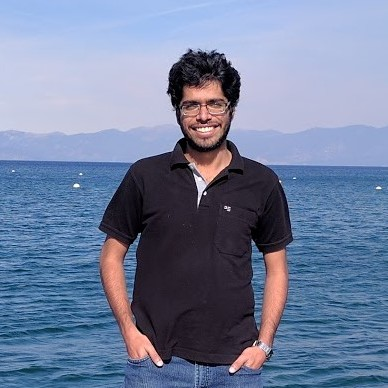
\includegraphics[width=0.18\textwidth]{collaborators/sharan}
            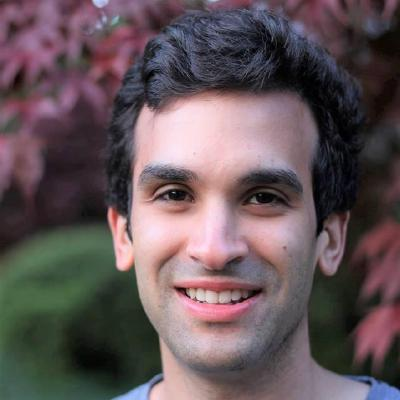
\includegraphics[width=0.18\textwidth]{collaborators/issam}
            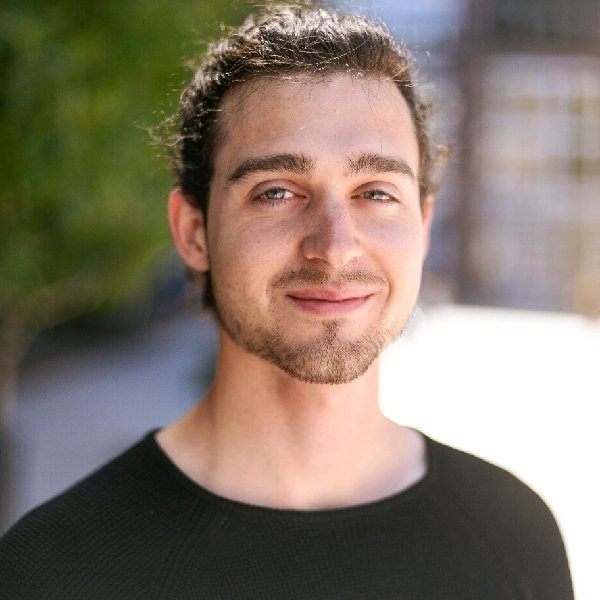
\includegraphics[width=0.18\textwidth]{collaborators/gauthier}
            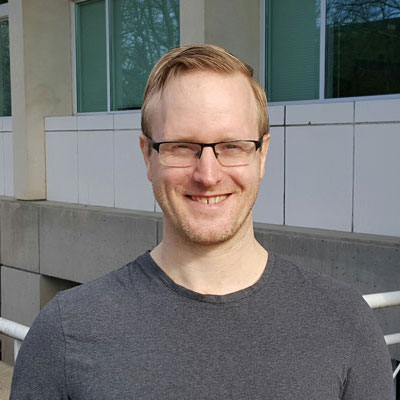
\includegraphics[width=0.18\textwidth]{collaborators/mark}
            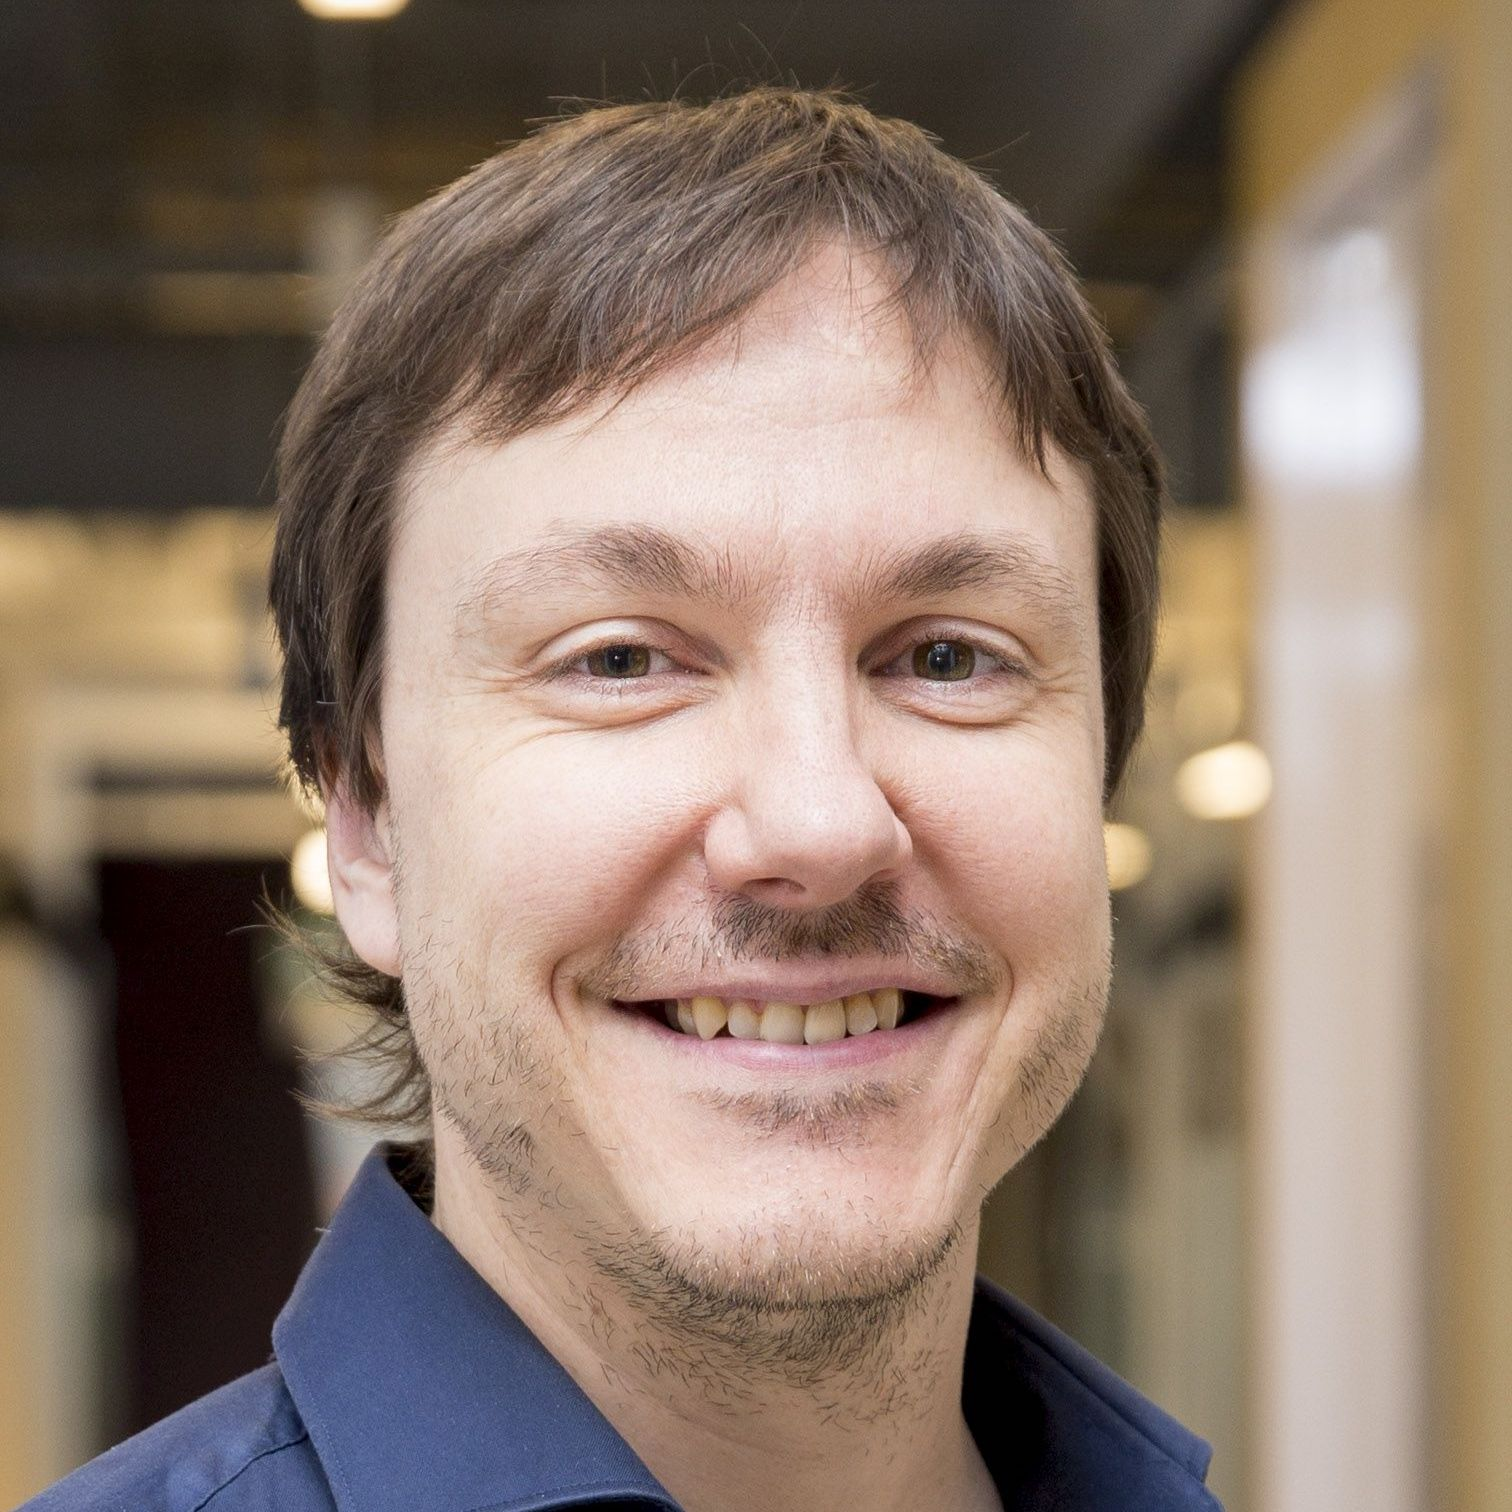
\includegraphics[width=0.18\textwidth]{collaborators/simon}

            \vspace{0.4ex}%

            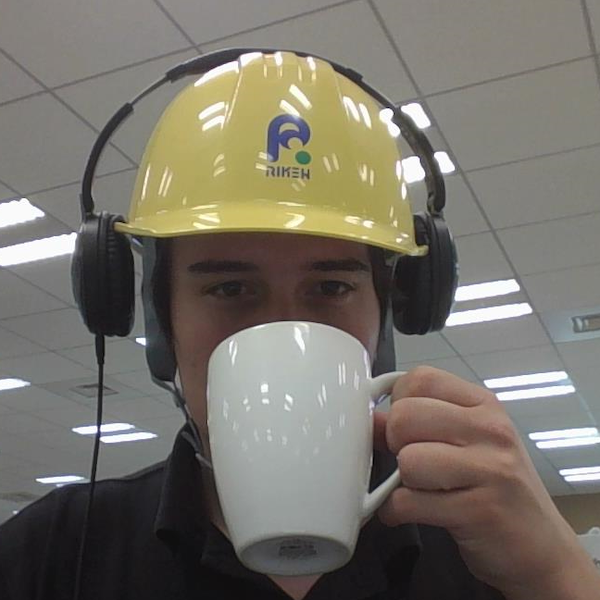
\includegraphics[width=0.18\textwidth]{collaborators/fred}
            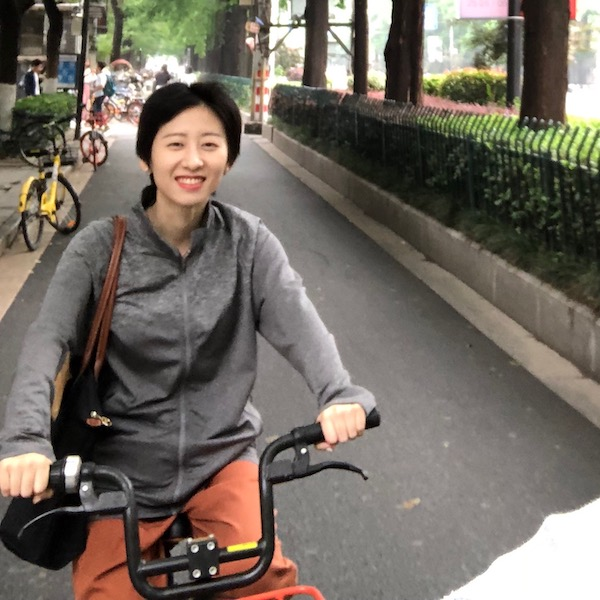
\includegraphics[width=0.18\textwidth]{collaborators/cathy}
            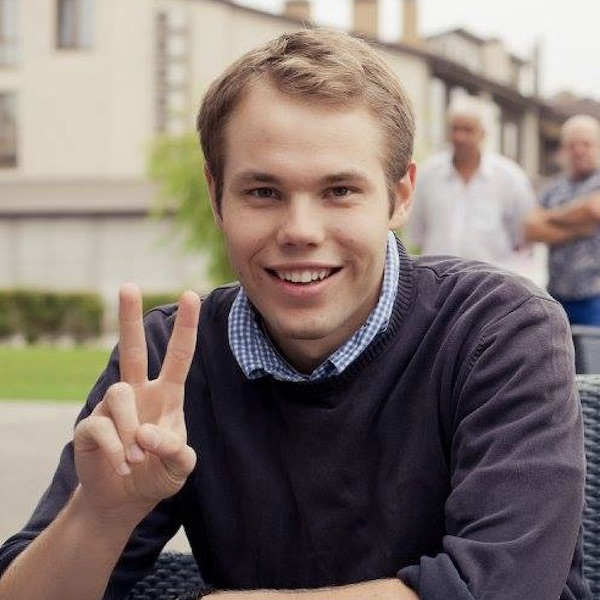
\includegraphics[width=0.18\textwidth]{collaborators/wilder}
            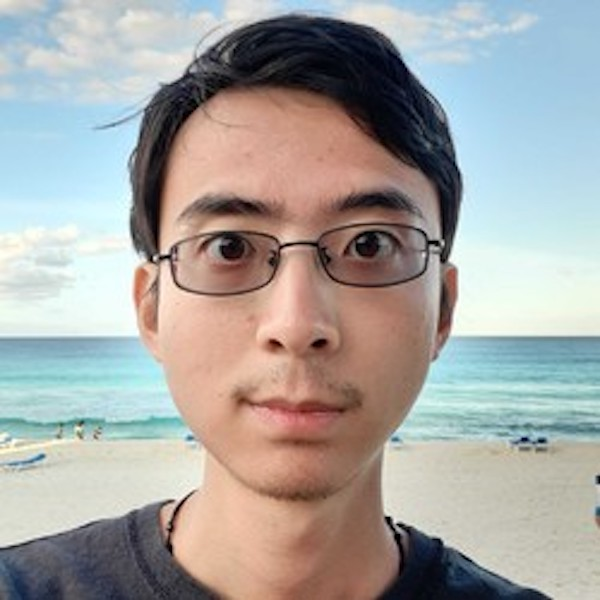
\includegraphics[width=0.18\textwidth]{collaborators/joey}
        \end{figure}

    \end{frame}
   
    \setbeamercolor{background canvas}{bg=white}
    
    \begin{frame}{Motivation: Model Fitting}
       \begin{center}
         Training Bayesian neural networks is dangerous work! 
       \end{center}
       
       \begin{figure}
            \centering
            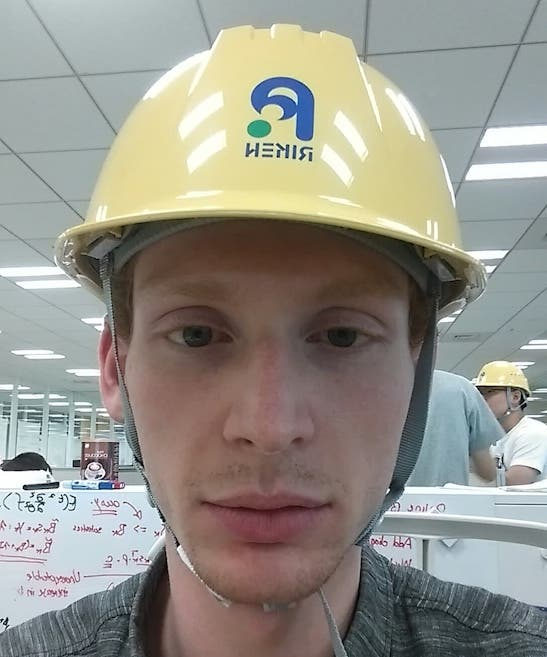
\includegraphics[width=0.45\textwidth]{collaborators/helmet1} 
            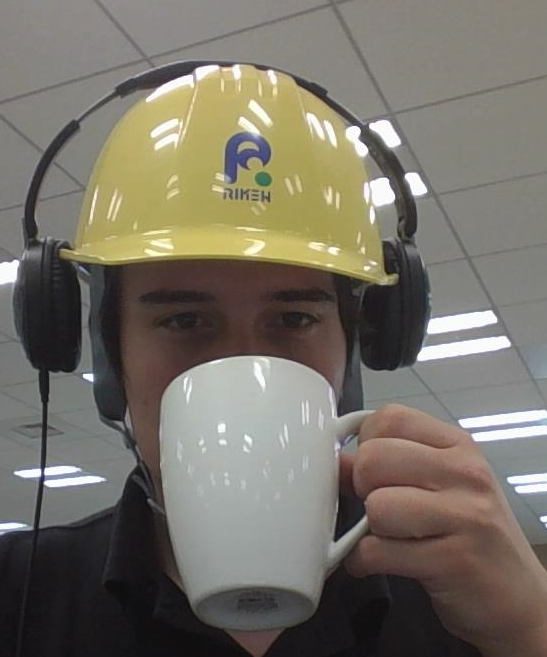
\includegraphics[width=0.45\textwidth]{collaborators/helmet2} 
       \end{figure} 
    \end{frame}

    \begin{frame}{Motivation: Model Fitting in ML}
       
       \begin{figure}
            \centering
            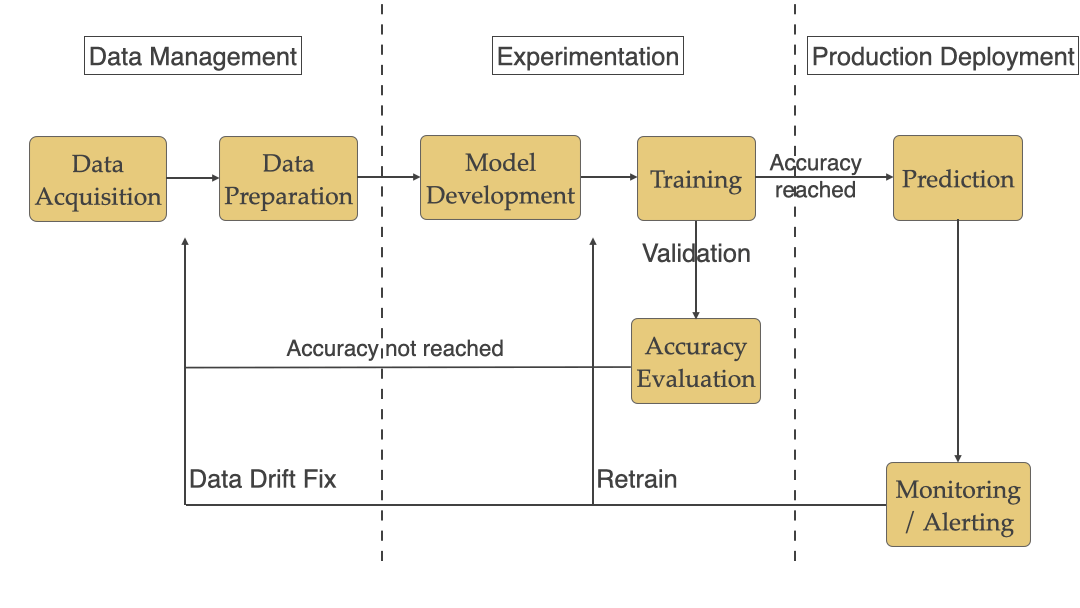
\includegraphics[width=0.98\textwidth]{figures/workflow} 
       \end{figure} 

       \source{https://towardsdatascience.com/challenges-deploying-machine-learning-models-to-production-ded3f9009cb3}
    \end{frame}

    \begin{frame}{Motivation: Model Fitting in ML}
       
       \begin{figure}
            \centering
            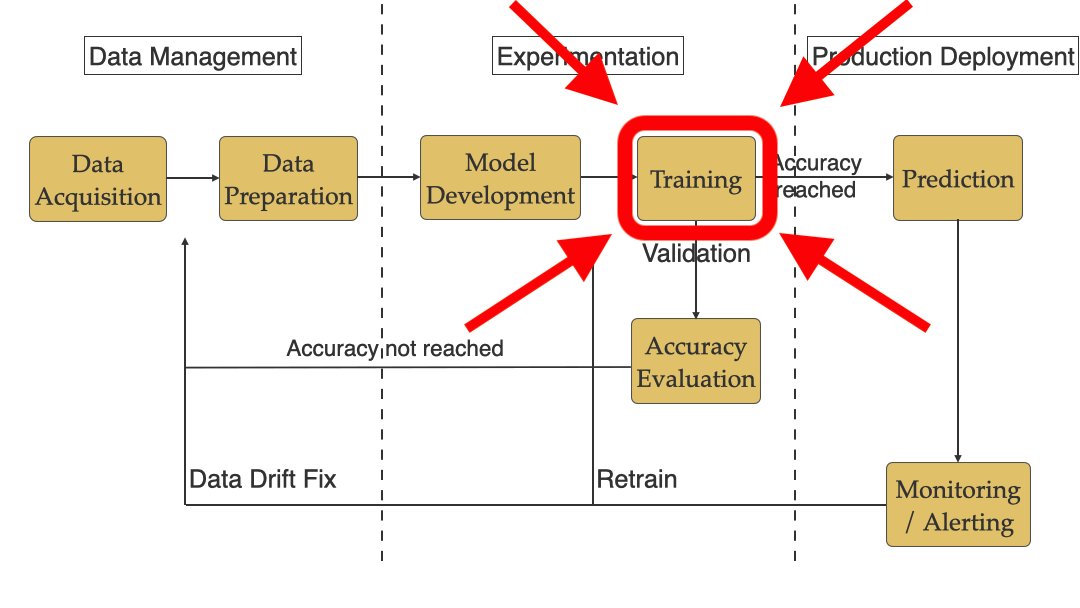
\includegraphics[width=0.98\textwidth]{figures/workflow_highlighted} 
       \end{figure} 

       \source{https://towardsdatascience.com/challenges-deploying-machine-learning-models-to-production-ded3f9009cb3}
    \end{frame}
    
    \begin{frame}{Motivation: Stochastic Gradient Descent}

        \begin{center}
            \Large
            ``Stochastic gradient descent (SGD) is today one of the main workhorses for solving large-scale supervised learning and optimization problems.''\\
            ---\citet{drori2019complexity}
        \end{center}

    \end{frame}

    \begin{frame}{Motivation: Consensus Says\ldots}

        \begin{center}
            \Large \dots and also~\citet{xu2017second,
            zhang2016parallel,
            patterson2017deep,
            pillaud2018statistical,
            grosse2015scaling,
            assran2018stochastic,
            damaskinos2019aggregathor,
            kawaguchi2020ordered,
            bernstein2018signsgd,
            li2019rsa,
            agarwal2017second,
            hofmann2015variance,
            geffner2019rule,
            assran2020convergence,
            gower2019sgd}
        \end{center}

    \end{frame}

    \begin{frame}{Motivation: Challenges in Optimization for ML}

        \textbf{Stochastic gradient methods} are the most popular algorithms for fitting ML models,
        \begin{align*}
            \textbf{SGD:} \quad w_{k + 1} = w_k - \eta_k \nabla f_i \, (w_k). \\
        \end{align*}

        % SGD is scalable and converges if $\eta_k$ decreases sufficiently slowly.\vspace{1em}

        But practitioners face major challenges with \vspace{0.5em}
        \begin{itemize}
            \item \textbf{Speed}: step-size/averaging controls convergence rate.
            \item \textbf{Stability}: hyper-parameters must be tuned carefully.
            \item \textbf{Generalization}: optimizers encode statistical tradeoffs.
        \end{itemize}
        \vspace{1em}

    \end{frame}

    \begin{frame}{Better Optimization via Better Models}

        \begin{figure}
            \centering
            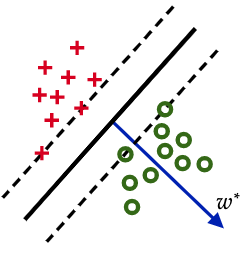
\includegraphics[width=0.38\textwidth]{figures/separable}
            \hspace{0.2em}
            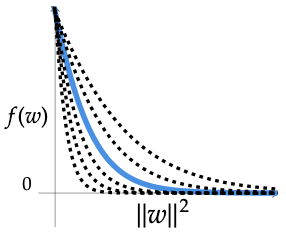
\includegraphics[width=0.45\textwidth]{figures/loss_fn}
        \end{figure}
        \vspace{0.2em}

        \begin{center}
            \large \textbf{Idea}: exploit over-parameterization for better optimization.\vspace{0.25em}
        \end{center}

    \end{frame}


    \begin{frame}{Interpolation}
        
    \end{frame}

    \begin{frame}{Growth Conditions}
        
    \end{frame}

    \begin{frame}{Stochastic Gradient Descent}
        
    \end{frame}
    
    \begin{frame}{Line Search}
        
    \end{frame}

    \begin{frame}{Acceleration}
        
    \end{frame}

    %% end slide
    \setbeamercolor{background canvas}{bg=lightcyan}

    \begin{frame}{}
        \begin{center}
        \huge Thanks for Listening!
        \end{center}
    \end{frame}

    \setbeamercolor{background canvas}{bg=white}

    \begin{frame}{Acknowledgements}
        I owe a great debt to my collaborators (left to right):
        \begin{center}    
            \href{https://vaswanis.github.io/}{Sharan Vaswani}, \href{https://issamlaradji.github.io/}{Issam Laradji}, \href{https://gauthiergidel.github.io/}{Gauthier Gidel}, \href{https://www.cs.ubc.ca/~schmidtm/}{Mark Schmidt}, \href{http://www.iro.umontreal.ca/~slacoste/}{Simon Lacoste-Julien}, \href{https://fkunstner.github.io/}{Frederik Kunstner}, \href{https://www.cs.ubc.ca/~mengxixi/}{Si Yi Meng}, \href{https://wilderlavington.github.io/}{Jonathan Lavington}, \href{https://joeyandbluewhale.github.io/}{Yihan Zhou}, and Betty Shea (not pictured). 
        \end{center}
        
        \begin{figure}
            \centering
            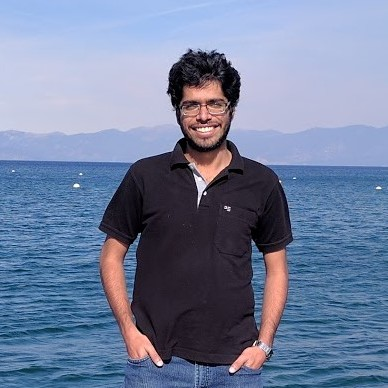
\includegraphics[width=0.18\textwidth]{collaborators/sharan}
            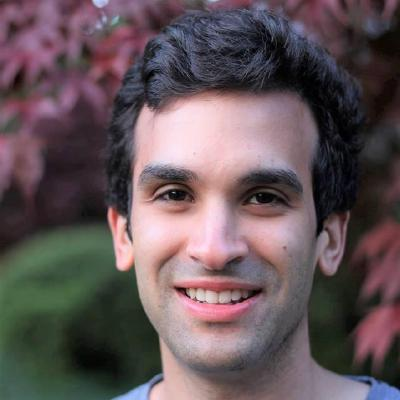
\includegraphics[width=0.18\textwidth]{collaborators/issam}
            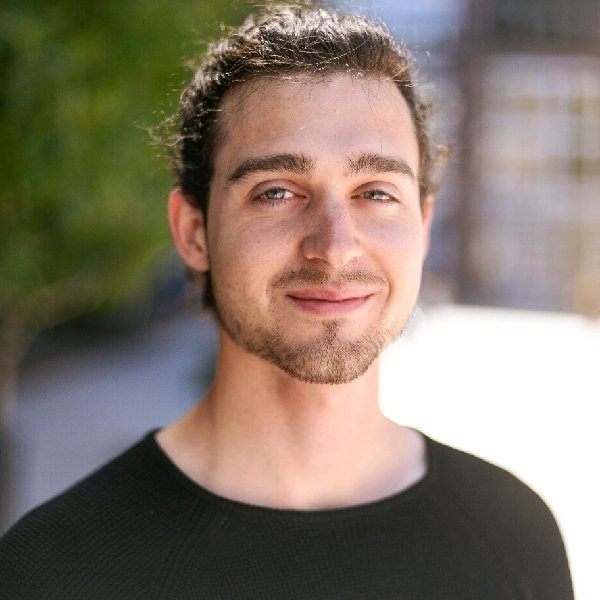
\includegraphics[width=0.18\textwidth]{collaborators/gauthier}
            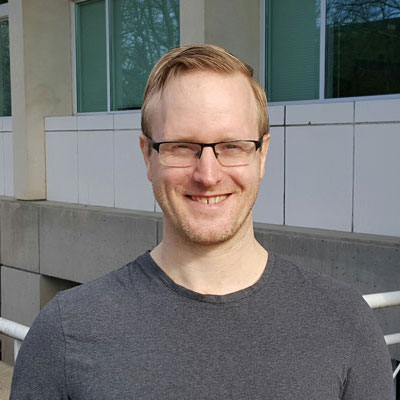
\includegraphics[width=0.18\textwidth]{collaborators/mark}
            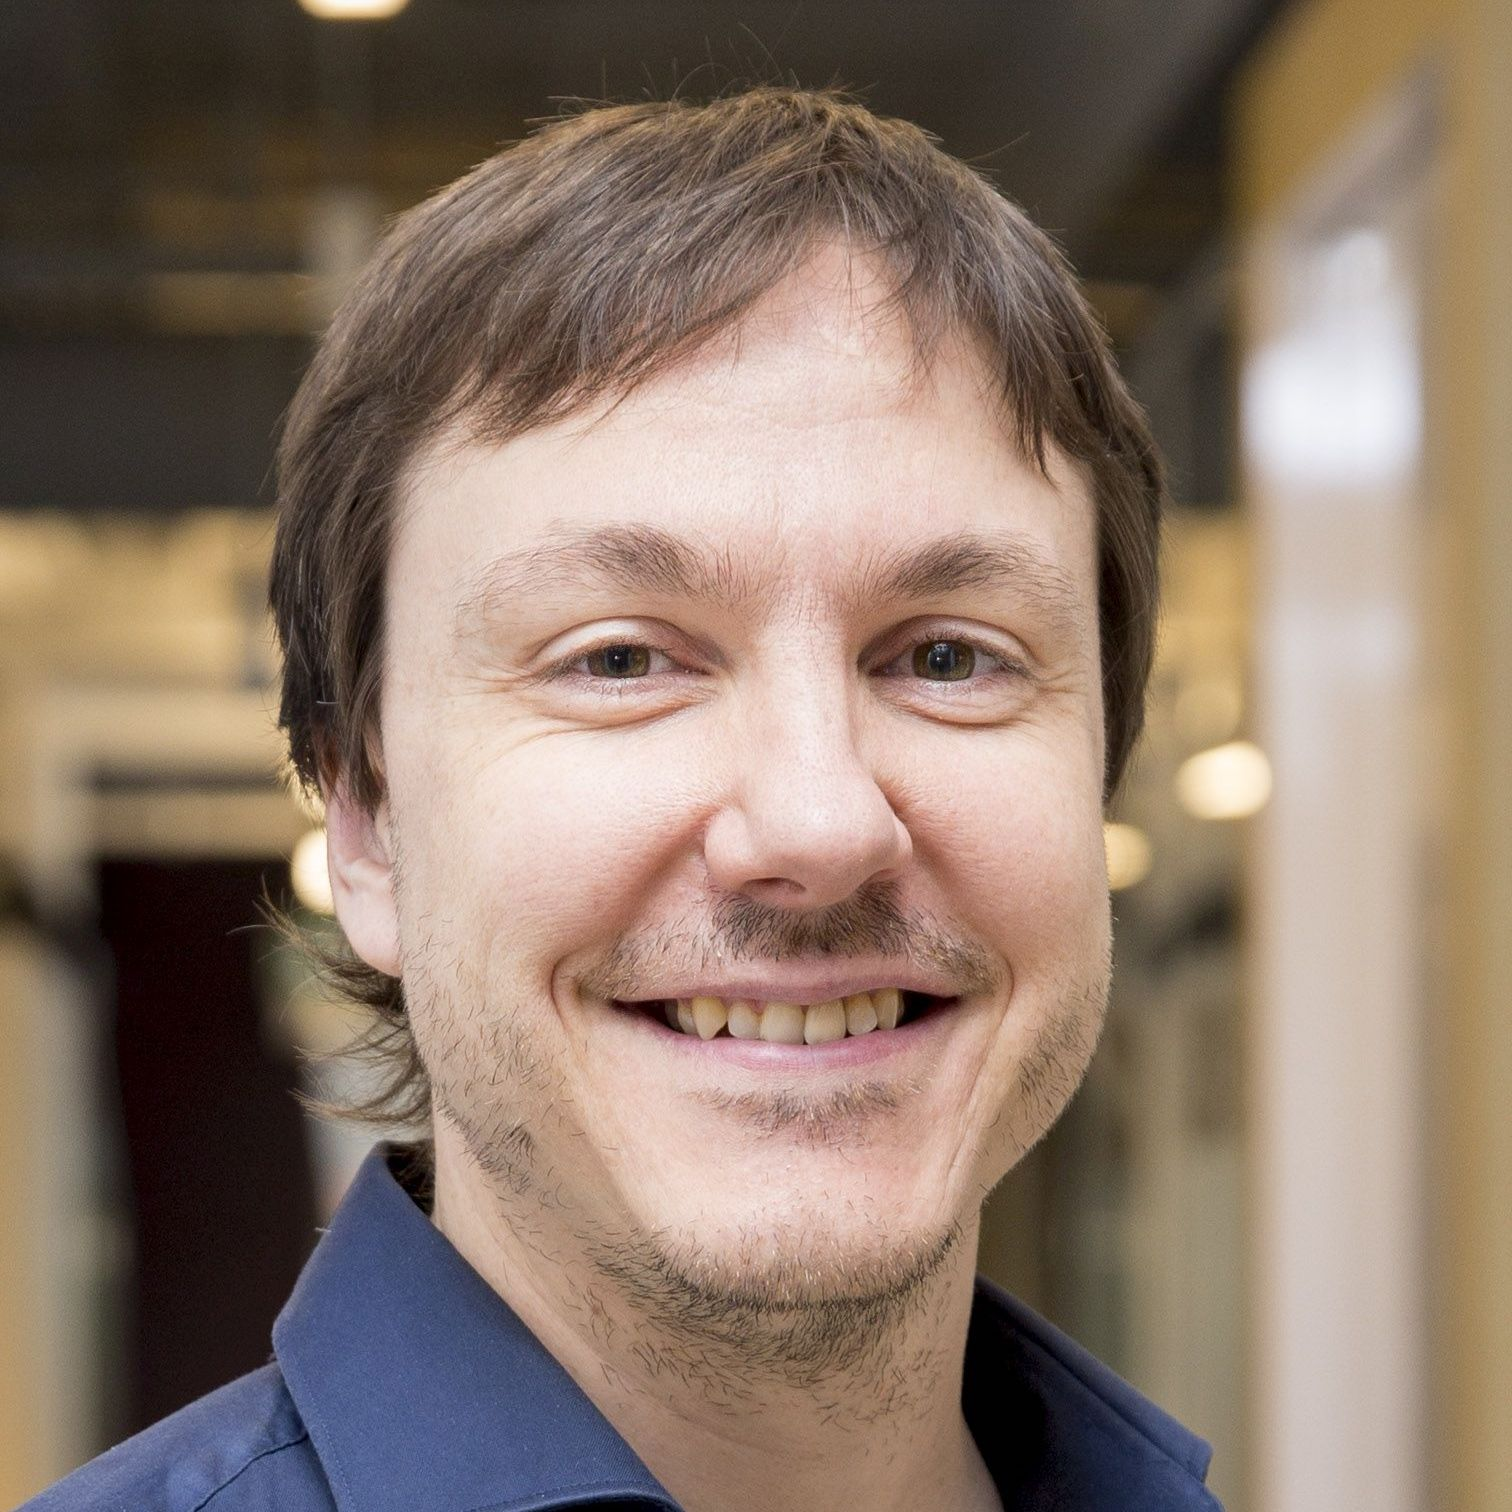
\includegraphics[width=0.18\textwidth]{collaborators/simon}

            \vspace{0.4ex}%

            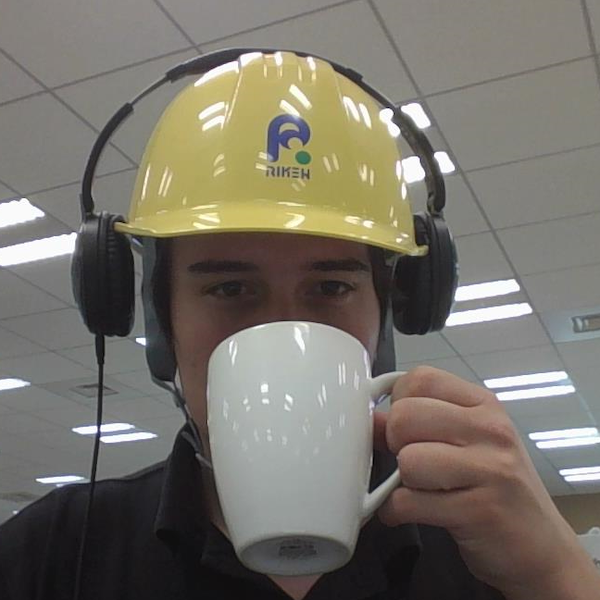
\includegraphics[width=0.18\textwidth]{collaborators/fred}
            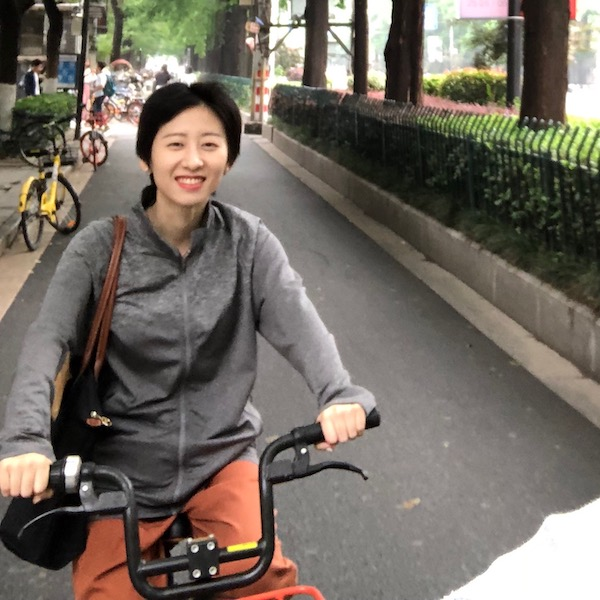
\includegraphics[width=0.18\textwidth]{collaborators/cathy}
            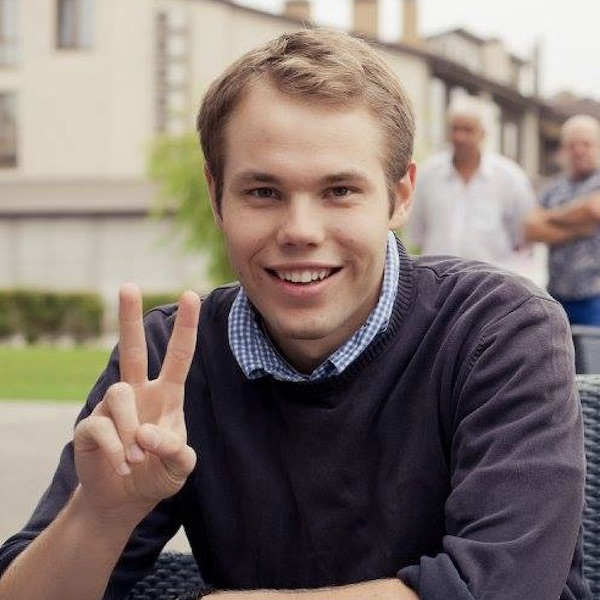
\includegraphics[width=0.18\textwidth]{collaborators/wilder}
            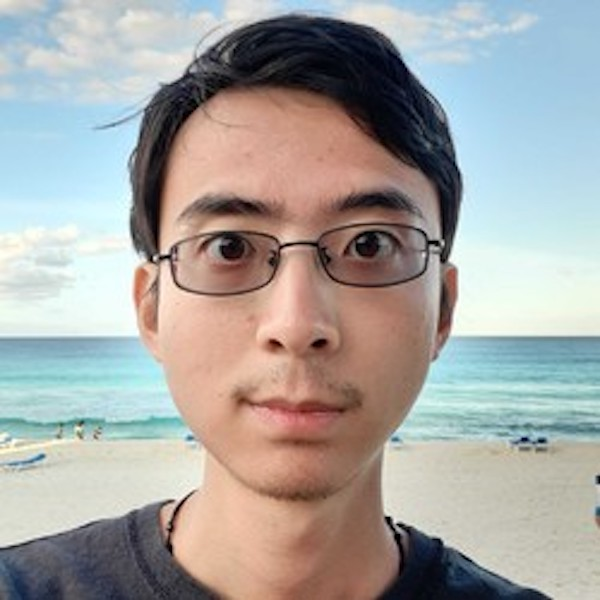
\includegraphics[width=0.18\textwidth]{collaborators/joey}
        \end{figure}

    \end{frame}

    %% bibliography
    \begin{frame}[allowframebreaks]{References}
        \bibliographystyle{plainnat}
        \bibliography{refs}
    \end{frame}


\end{document}
